\documentclass[preview]{standalone}

\usepackage{amsmath}
\usepackage{amssymb}
\usepackage{stellar}
\usepackage{bettelini}

\hypersetup{
    colorlinks=true,
    linkcolor=black,
    urlcolor=blue,
    pdftitle={Biologia},
    pdfpagemode=FullScreen,
}

\begin{document}

\title{Biologia}
\id{biologia-sistema-digerente-e-nutrizione}
\genpage

\begin{snippet}{trasformazione-cibo-expl1}
    La trasformazione del cibo avviene in quattro fasi distinte.
    \begin{enumerate}
        \item \textbf{ingestione;}
        \item \textbf{digestione:} demolizione del cibo. Viene convertito in molecole sempre più piccole per essere
        assorbite dal corpo. La maggior parte delle molecole che costituiscono il cibo sono
        biomolecole e sono grandi;
        \item \textbf{assorbimento:} avviene grazie alle cellule che rivestono il tubo digerente.
        Le molecole vengono scomposte in piccoli pezzi come aminoacidi o piccoli zuccheri;
        \item \textbf{eliminazione:} scarti che vengono
        espulsi dal tubo digerente.
    \end{enumerate}

    Tutto parte dal tubo digerente e delle ghiandole a esso associate:
    Ghiandole salivali, pancreas e fegato. I denti e la lingua sono organi
    della cavità orale e sono annessi al sistema digerente.
    Il cibo introdotto dalla bocca e masticato dai denti viene spinto dalla
    lingua alla faringe.
\end{snippet}

\begin{snippetdefinition}{peristalsi-definizione}{Peristalsi}
    La \textit{peristalsi} è un processo in cui ci sono delle onde di
    contrazione e rilassamento dei muscoli lisci presenti nella
    parete del tubo digerente.
\end{snippetdefinition}

\begin{snippet}{trasformazione-cibo-espl2}
    Dopo essere stato deglutito viene sospinto dal
    processo di peristalsi.
    \\
    In una decina di secondi il cibo passa dall'esofago allo stomaco. Due
    valvole muscolari, chiamate sfinteri, regolano il passaggio del cibo.
    
    \begin{enumerate}
        \item Il cardias regola il passaggio dall'esofago allo stomaco
        \item Il piloro regola il passaggio dallo stomaco all'intestino tenue
        Il piloro permette al cibo di rimanere chiuso nello stomaco dalle.
        2 alle 6 ore, così da permettere ai succhi gastrici e agli enzimi
        di cominciare la digestione
    \end{enumerate}
    
    La fase finale della digestione e l'assorbimento avvengono
    nell'intestino tenue nell'arco di 5-6 ore. Le sostanze non digerite
    continuano nell'intestino crasso, l'acqua viene riassorbita e il restante
    si tramuta in feci che verranno poi espulse. Per questo processo ci
    vogliono dalle 12 alle 24 ore.
\end{snippet}

\section{Bocca}

\begin{snippet}{203f5a74-b90e-47d8-b278-eacae6123c4b}
    La secrezione che si trova all'interno della bocca è la saliva e l'enzima
    presente è l'\textit{amilasi salivare}.
    Sono presenti altre sostanze come la mucina (il muco).
    L'amilasi salivare scompone l'amido in maltosio e destrine. (oligosaccaridi ?)
\end{snippet}

\begin{snippet}{tabella-illustration}
    \begin{center}
    \begin{figure}[th]
        \centering
        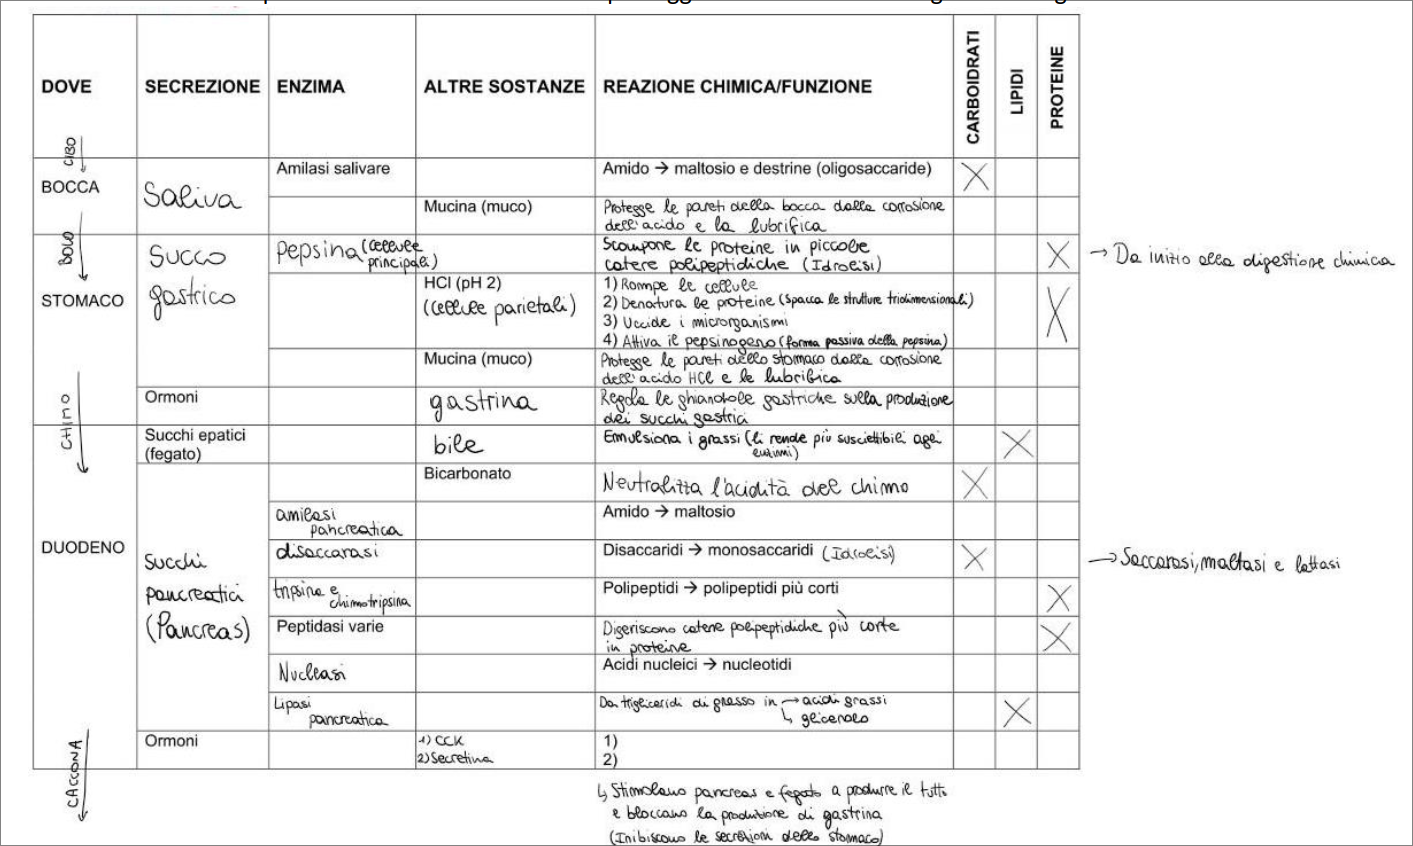
\includegraphics[width=\textwidth]{./resources/tabella.png}
    \end{figure}
    \end{center}
\end{snippet}

\section{Intesino}

\begin{snippet}{digestione-illustration}
    \begin{center}
    \begin{figure}[th]
        \centering
        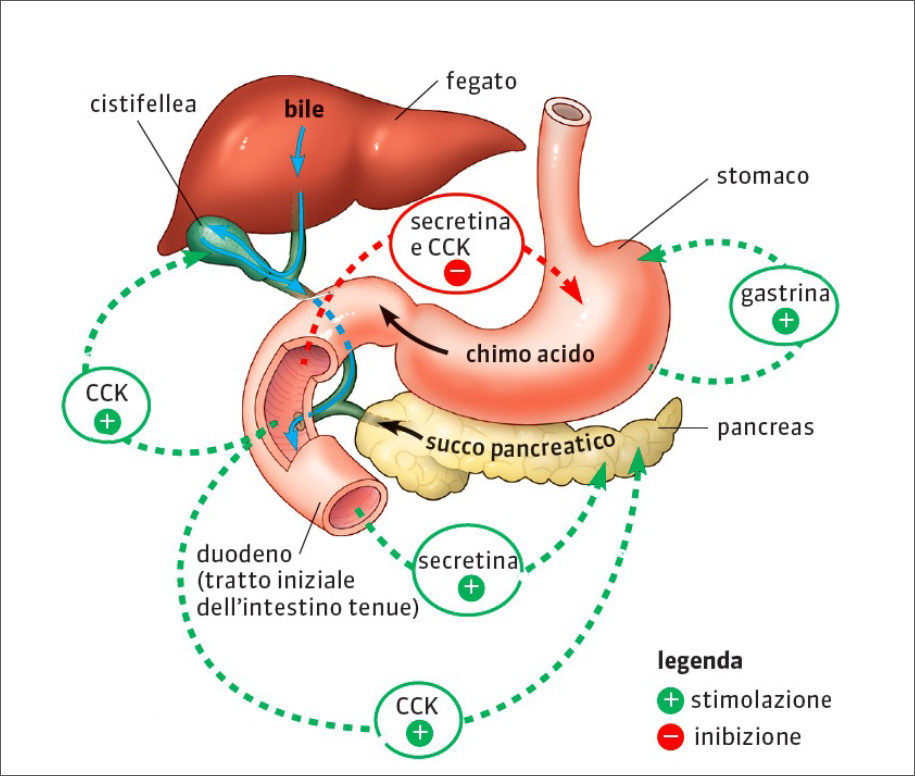
\includegraphics[width=0.5\textwidth]{./resources/digestione.png}
    \end{figure}
    \end{center}
\end{snippet}

\begin{snippet}{assorbimento-intestino-tenue}
    Nell'intestino tenue vengono assorbiti:
    \begin{itemize}
       \item Monosaccaridi
       \item Amminoacidi
       \item Acidi grassi e glicerolo
       \item Nucleotidi
       \item Vitamine
       \item Acqua
       \item Sali minerali
    \end{itemize}
\end{snippet}

\begin{snippet}{intestino-illustration}
    \begin{center}
    \begin{figure}[th]
        \centering
        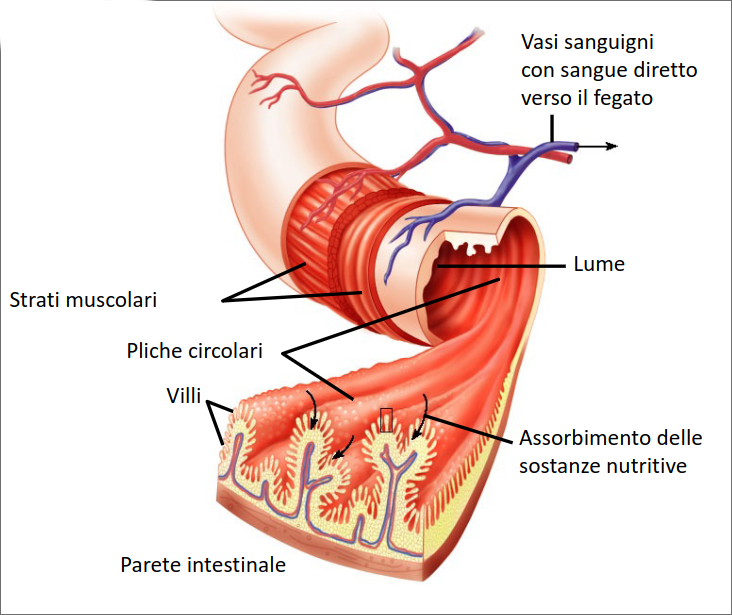
\includegraphics[width=0.75\textwidth]{./resources/intestino.png}
    \end{figure}
    \end{center}
\end{snippet}

\begin{snippet}{assorbimento-illustration}
    \begin{center}
    \begin{figure}[th]
        \centering
        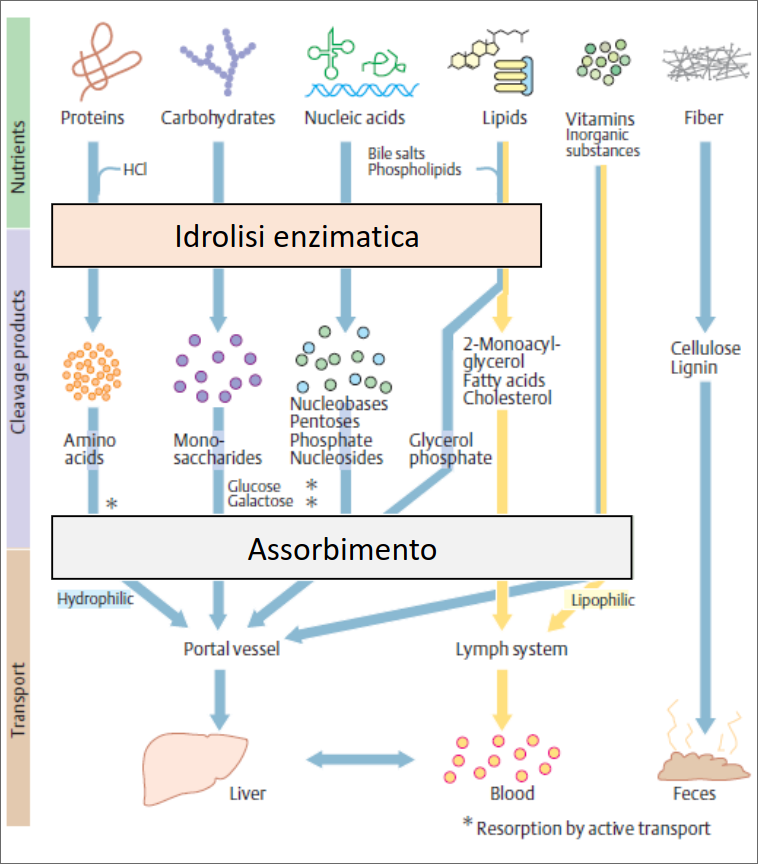
\includegraphics[width=\textwidth]{./resources/assorbimento.png}
    \end{figure}
    \end{center}
\end{snippet}

\plain{Le fibre non hanno un vero valore nutrizionale ma permettono un miglior assorbimento delle sostanze fibrose.}

\begin{snippet}{nutrizione-illustration}
    \begin{center}
    \begin{figure}[th]
        \centering
        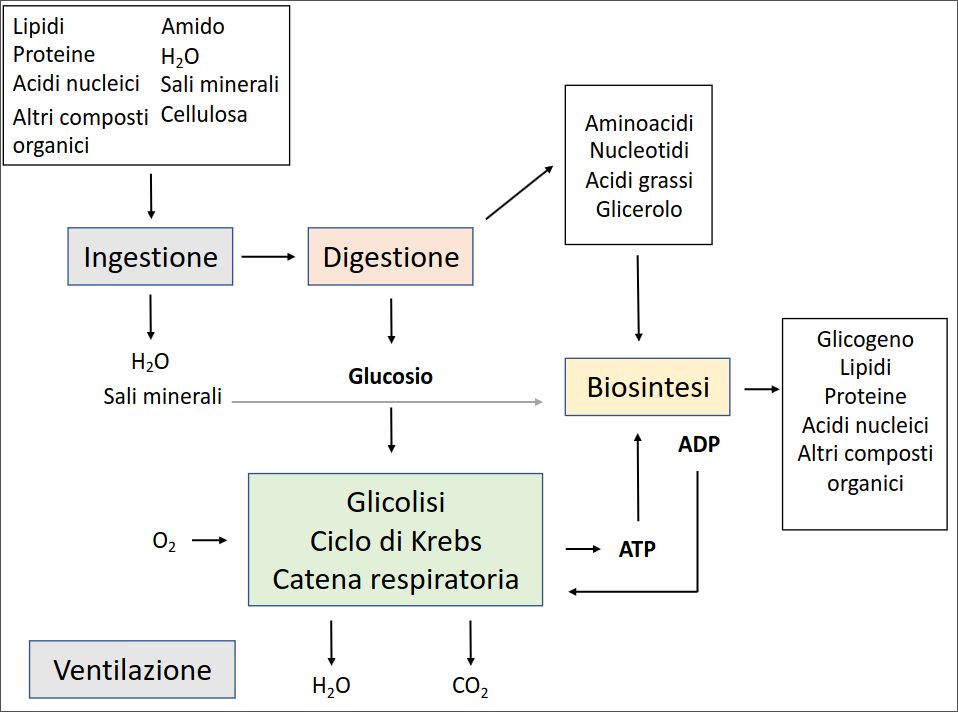
\includegraphics[width=\textwidth]{./resources/nutrizione.png}
    \end{figure}
    \end{center}
\end{snippet}

\begin{snippet}{f4e3df87-8041-42ac-8ead-2a4f7ef1683e}
    Otto amminoacidi su 20 sono essenziali, e per cui devono per forza essere assorbiti dall'alimentazione
siccome non possono essere prodotti. 
Se la cellula non necesita di amminoacidi, essi vanno principalmente al fegato, il quale si occupa
di sfruttare questa materia organica in eccesso, ossia convertendola in glucosio o lipidi.
\end{snippet}

\begin{snippet}{protein-metabolism-illustration}
    \begin{center}
    \begin{figure}[th]
        \centering
        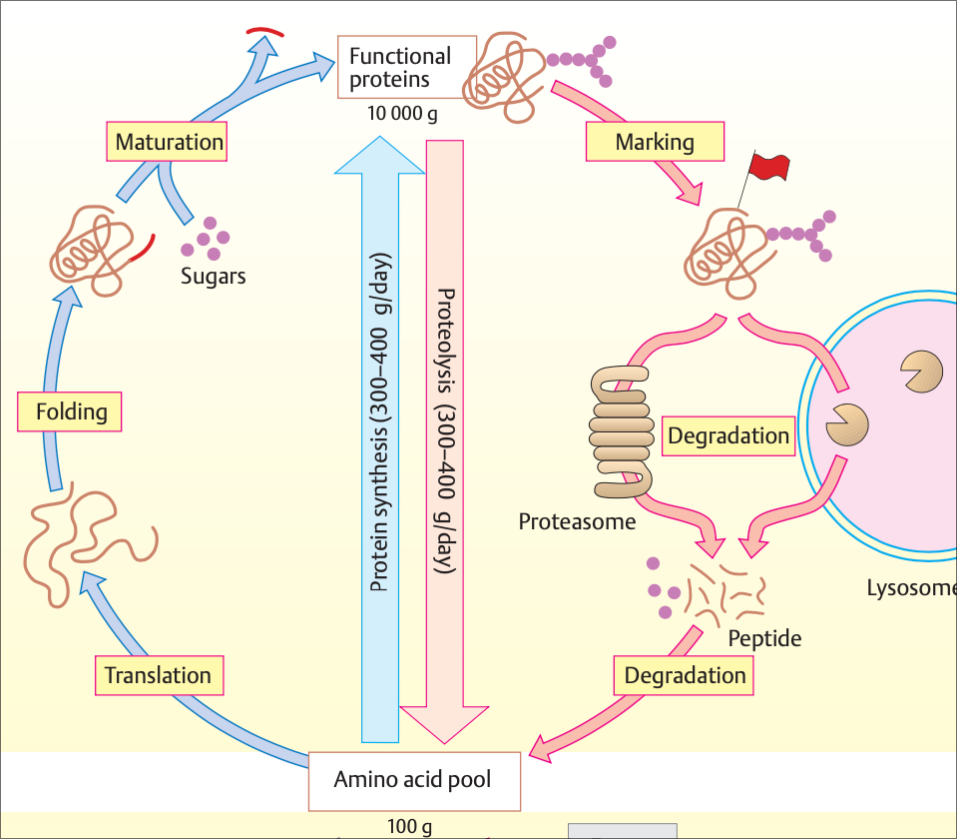
\includegraphics[width=0.6\textwidth]{./resources/protein_metabolism.png}
    \end{figure}
    \end{center}
\end{snippet}

\begin{snippet}{daily-intake-illustration}
    \begin{center}
    GDA per un adulto che si basano su un consumo giornaliero di $2000 \mathrm{kcal}$ (Calorie)
    \begin{tabular}{|l|r|}
    \hline Energia & GDA per adulti \\
    \hline Grassi totali & 2000 kcal (Calorie) \\
    \hline Grassi saturi & Non piú di $70 \mathrm{~g}$ \\
    \hline Carboidrati & Non più di $20 \mathrm{~g}$ \\
    \hline Zuccheri totali & $270 \mathrm{~g}$ \\
    \hline Proteine & Non più di $90 \mathrm{~g}$ \\
    \hline Fibro & $50 \mathrm{~g}$ \\
    \hline Sodio (Sale) & Almeno $25 \mathrm{~g}$ \\
    \hline
    \end{tabular}
    \end{center}
    \phantom{}
\end{snippet}

\plain{Il corpo ha bisogno anche di determinati tipi di elementi per svolgere determinate tipi di funzioni.}

\begin{snippetdefinition}{metabolismo-basale-definizione}{Metabolismo basale}
    Con \textit{metabolismo basale} si intende la quantità di energia impiegata in condizioni di neutralità termica.
\end{snippetdefinition}

\end{document}